\documentclass[fleqn,10pt]{wlscirep}
\usepackage[utf8]{inputenc}
\usepackage[T1]{fontenc}

\title{Scientific Reports Title to see here}

\author[1,*]{Alice Author}
\author[2]{Bob Author}
\author[1,2,+]{Christine Author}
\author[2,+]{Derek Author}

\affil[1]{Affiliation, department, city, postcode, country}
\affil[2]{Affiliation, department, city, postcode, country}

\affil[*]{corresponding.author@email.example}
\affil[+]{these authors contributed equally to this work}

\keywords{Keyword1, Keyword2, Keyword3}

\begin{abstract}
Example Abstract. Abstract must not include subheadings or citations. Example Abstract. Abstract must not include subheadings or citations. Example Abstract. Abstract must not include subheadings or citations. Example Abstract. Abstract must not include subheadings or citations. Example Abstract. Abstract must not include subheadings or citations. Example Abstract. Abstract must not include subheadings or citations. Example Abstract. Abstract must not include subheadings or citations. Example Abstract. Abstract must not include subheadings or citations.
\end{abstract}
\begin{document}

\flushbottom
\maketitle

\thispagestyle{empty}

\noindent Please note: Abbreviations should be introduced at the first mention in the main text – no abbreviations lists. Suggested structure of main text (not enforced) is provided below.

\section*{Introduction}

The Introduction section, of referenced text \cite{Tesniere18} expands on the background of the work (some overlap with the Abstract is acceptable). The introduction should not include subheadings \cite{galeote_genome+sequence+of+torulaspora+microellipsoides+clib+830t_2018}.

\section*{Results}

Up to three levels of \textbf{subheading} are permitted. Subheadings should not be numbered.

\subsection*{Subsection}

Example text under a subsection. 

\subsubsection*{Subsubsection}
 
Topical subheadings are allowed. Figure \ref{fig:figure1} is referenced here.

\section*{Discussion}

The Discussion should be succinct and must not contain subheadings.

\section*{Methods}

Topical subheadings are allowed. Authors must ensure that their Methods section includes adequate experimental and characterization data necessary for others in the field to reproduce their work.

\bibliography{sample}

\section*{Acknowledgements (not compulsory)}

Acknowledgements should be brief, and should not include thanks to anonymous referees and editors, or effusive comments. Grant or contribution numbers may be acknowledged.

\section*{Author contributions statement}

Must include all authors, identified by initials, for example:
A.A. conceived the experiment(s),  A.A. and B.A. conducted the experiment(s), C.A. and D.A. analysed the results.  All authors reviewed the manuscript. 

\section*{Additional information}

To include, in this order: \textbf{Accession codes} (where applicable); \textbf{Competing interests} (mandatory statement). 

The corresponding author is responsible for submitting a \href{http://www.nature.com/srep/policies/index.html#competing}{competing interests statement} on behalf of all authors of the paper. This statement must be included in the submitted article file.

Figures and tables can be referenced in LaTeX using the ref command, e.g. Figure \ref{fig:figure1} and Table \ref{tab:example}.

\begin{figure}[ht]
\centering
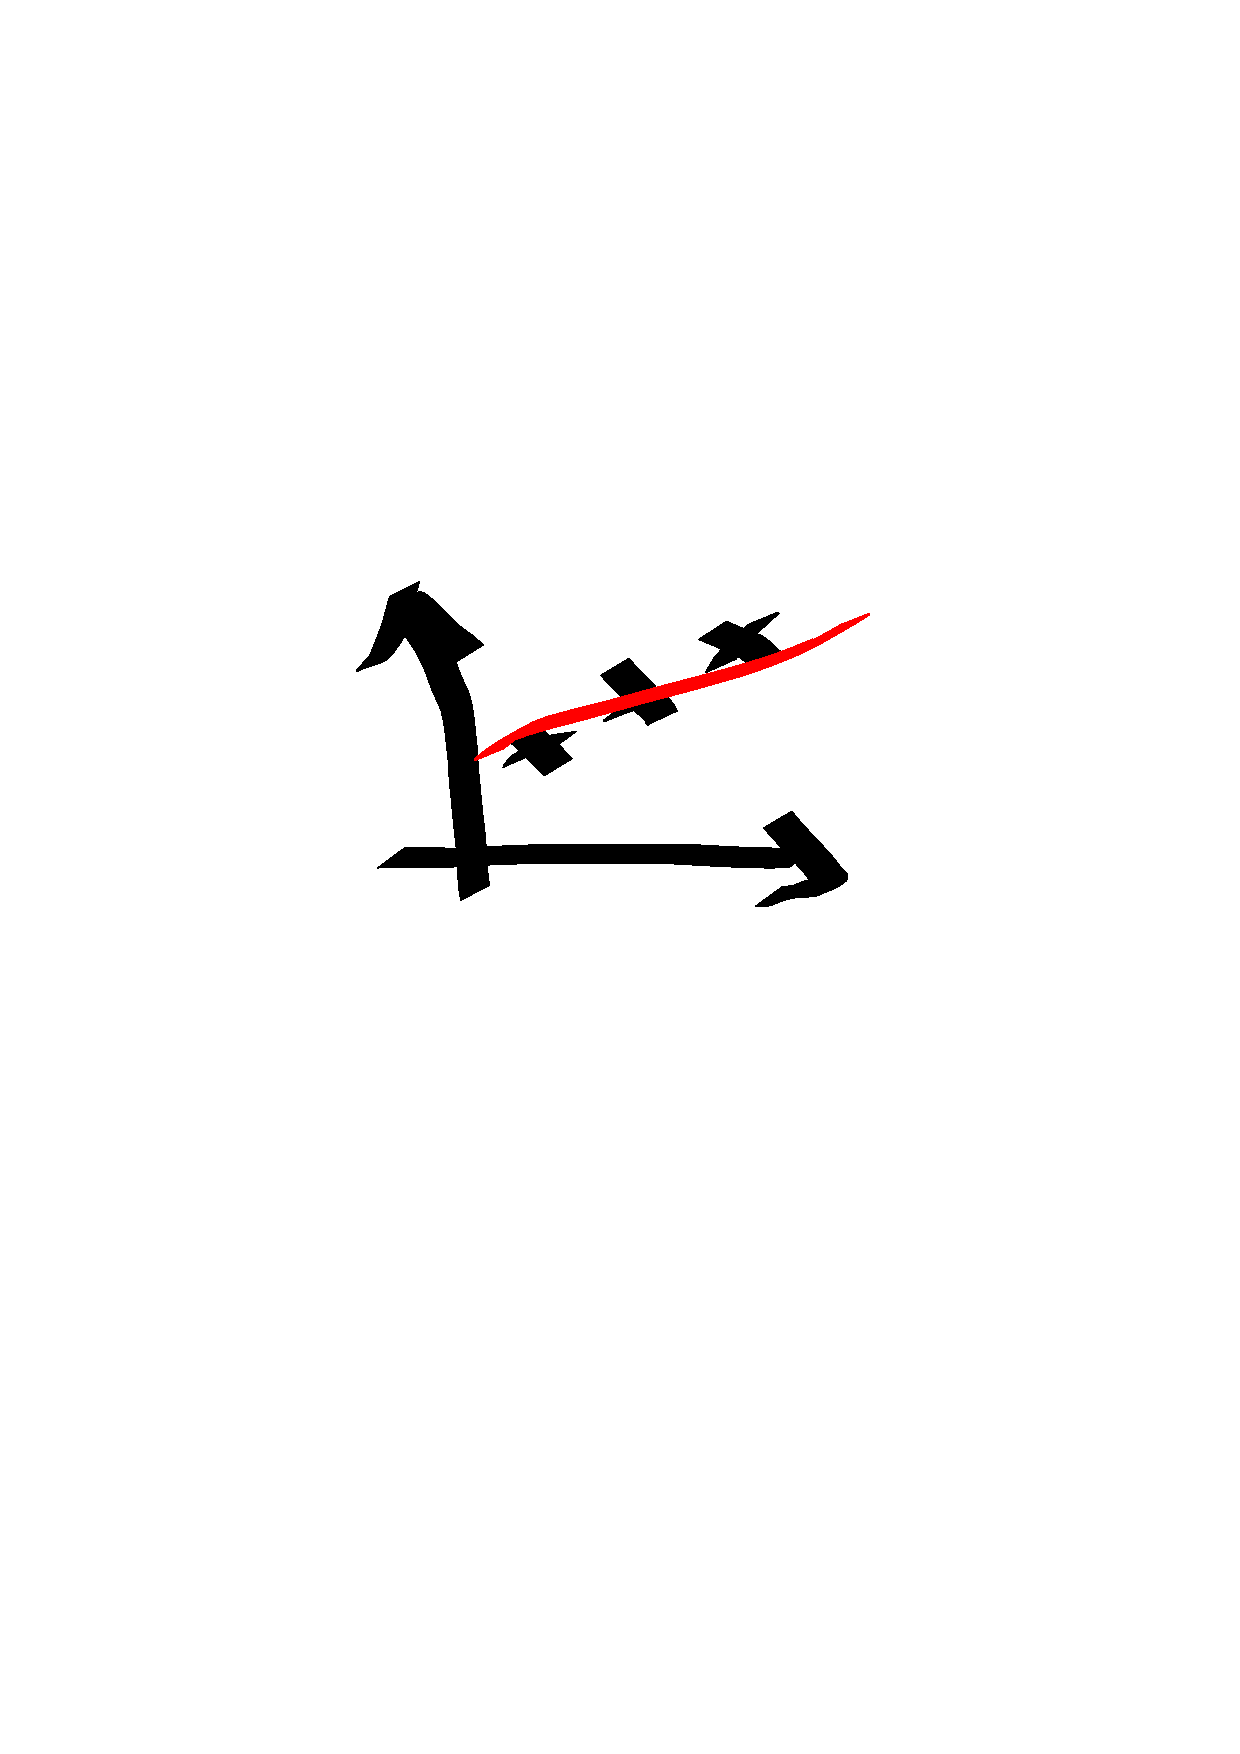
\includegraphics[width=0.75\linewidth]{Figure1.pdf}
\caption{Legend (350 words max). Example legend text.}
\label{fig:figure1}
\end{figure}

\begin{table}[ht]
\centering
\begin{tabular}{lll}
\hline
Condition & n & p \\
\hline
A & 5 & 0.1 \\
B & 10 & 0.01 \\
\hline
\end{tabular}
\caption{\label{tab:example}Legend (350 words max). Example legend text.}
\end{table}

\end{document}